\NextFile{details.html}

\chapter{Little Details} \label{chap:details}

Most readers may wish to skip this chapter, in which we discuss the finer
points of a few important aspects of 3D printing.  These points are not
unique to Sailfish and apply to 3D printing in general, although the
terminology may differ from printer to printer, as from firmware to firmware.

Understanding of the material in this chapter is not critical to successful
3D printing.  However, at some point in your 3D printing career, you may
find something here which answers a nagging question.  Or not.

\NextFile{details-z-home-offset.html}

\section{Z Home Offset} \label{sec:z-home-offset}
\index{Home offsets!Z}
\index{Offsets!Z}

The Z home offset plays a critical role in the success of your print.  Namely,
it influences a print's first layer whose proper adhesion to the build plate
is critical.  When the first layer is too far from the build plate,
the print will not properly adhere and may detach mid-print, destroying
the build.  And, if the first layer is too close to the build plate, the
extruder may jam.

How does the Z home offset affect this?  If you are not using
software-based auto-leveling, then it does so by defining the initial
position of the build plate.\footnote{For software-based auto-leveling, refer
to Section~\ref{sec:auto-leveling}.} Typically, the Z home offset has
the value 0 and thus states that after homing, the build plate is at
position Z=0.  More generally, after homing the build plate is at the
position

\begin{equation*}
Z=H_z,
\end{equation*}

where $H_z$ is the value of the Z home offset.

When you slice a model, your slicer generates instructions which place the
first layer at an initial height, $Z_i$.  This height will not be zero.
Rather it is some height larger than zero; often it is one-half the
layer height, but that varies between slicers and is often
configured in your slicing ``profile''.

To complete our mental picture of the first layer height, we must finally
take into account the small gap we created between the tip of the nozzle
and the top of the build plate when we leveled (``trammed'') the build
plate.  Often we use a sheet of paper, whose thickness is about 0.1~mm.
This small gap must also be taken into account.  Let us use the symbol $g$
to represent the size of this gap.  See Figure~\ref{fig:zhome} for a
diagram of these values.

\begin{figure}[!htbp]
  \centering
    \ifpdf
      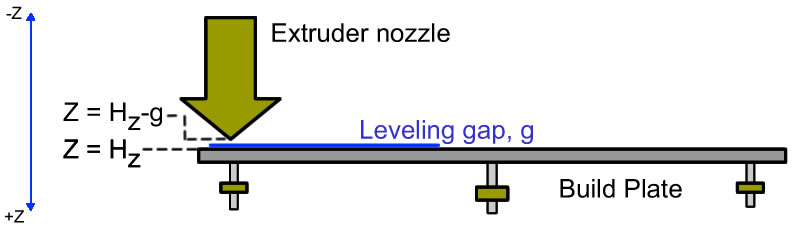
\includegraphics[width=5in]{z-home-offset}
    \else
      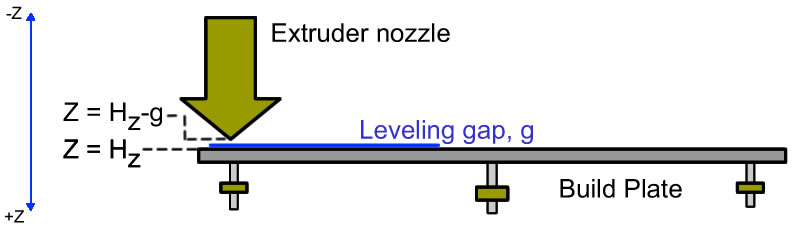
\includegraphics[width=7in]{z-home-offset}
    \fi
    \caption{The leveling gap, $g$}
  \label{fig:zhome}
\end{figure}

From Figure~\ref{fig:zhome} we see that after homing, the build plate is
at position $Z=H_z$ while the nozzle is actually at $Z=H_z-g$.  Note that
Z values \emph{decrease} as you move upwards in that diagram.  Increasing
print heights are had by lowering the build platform and thus moving
downward.  The distance between the build plate and nozzle in
Figure~\ref{fig:zhome} is the difference between their Z values,

\begin{equation*}
H_z-(H_z-g)
\end{equation*}

which simplifies, as we expect, to the value $g$, the gap.

With these values defined, we can now determine the critical vertical distance,
$D$, between the extruder nozzle and build plate for the first layer of a
print. It is

\begin{equation}\label{eq:D}
D=g + Z_i - H_z.
\end{equation}

That is, for the first layer the build plate is moved from its homed position
$H_z$ to the initial printing height, $Z_i$.  The vertical distance between
those two positions is $Z_i-H_z$.  Add to that the leveling gap, $g$, and
you have equation~\ref{eq:D}.  Alternatively, the value $D$ may be derived by
using the difference between the initial printing position $Z_i$ and the
extruder position (which remains fixed),

\begin{equation*}
Z_i-(H_z-g),
\end{equation*}

which again yields Equation~\ref{eq:D}.

For example, when $H_z=0$~mm, $g=0.1$~mm, and $Z_i=0.15$~mm, the initial
distance between the extruder and build plate is $0.25$~mm.

Now for the fun.  Suppose you are having a problem with a print not adhering
well and you know it needs to be started ever so slightly closer to the build
plate.  Your choices are to change the slicing profile and reslice ($Z_i$),
relevel the build plate with a smaller gap ($g$), or to adjust the
Z home offset ($H_z$).  Adjusting the Z home offset is quick and easy and
can be done from the printer's front display (Section~\ref{sec:homeoff}).
To decrease the initial distance, you wish to decrease $D$.  To do that,
\emph{increase} $H_z$.  For example, change it from $0$~mm to $0.03$~mm.
That causes $D$ to change from $0.25$~mm to $0.22$~mm and thus the initial
distance was decreased by $0.03$~mm.

Similarly, if you want to increase the initial distance, you can decrease
$H_z$.  Yes, it is okay to use a negative value for $H_z$.

In changing $H_z$, be careful to not change it too much.  Be careful to
not accidentally enter a large value such as $0.5$~mm.  You do not want
to generate a value of $D$ that is so small that you
damage your build plate, extruder, or both.

Finally, note that all slicers assume there is a slight leveling gap, $g$.
ReplicatorG and MakerWare assume a gap of approximately $0.1$~mm.  Other
slicers may assume a different leveling gap.  It is a good idea to learn
what gap your slicer assumes.  If you consistently have issues, it may
be that either you need to create a different leveling gap, or you should change your slicing profile to use the gap you have created.

\NextFile{details-toolhead-offsets.html}

\section{Toolhead Offsets} \label{sec:toolhead-offsets-detail}
\index{Toolhead offsets}
\index{Offsets!Toolhead}

For printers with two extruders, the firmware must effect a tool change when switching between extruders.  Part of this process entails moving the extruder you are about to use into the position currently occupied by the extruder you were using.  When switching from the right to the left extruder, this means moving the entire extruder carriage to the right.  And, when switching from the left to the right extruder, moving the carriage to the left.  The carriage needs to be moved forward or backwards as well when there is a displacement along the Y axis between the two extruders.

The distance along the X and Y axes which the carriage needs to be moved is the separation along those axes between the two extruders.  The separation along the X axis is referred to as the \emph{X toolhead offset}.  Similarly, the separation along the Y axis is the \emph{Y toolhead offset}.  Collectively, these values are referred to as the \emph{\glspl{toolhead offset}}.

For the next part, keep in mind that, while facing the front of the printer, the direction of increasing X is to the right and the direction of increasing Y is to the back.  The X toolhead offset is taken to be a positive distance.  Let us call this distance $O_x$.  The Y toolhead offset, $O_y$, is taken to be zero when the two extruders have no separation along the Y axis and positive when the left extruder is forward --- towards the front of the printer --- relative to the right extruder.  When switching from the right to left extruder, the carriage is thus moved by the displacement vector $(O_x, O_y)$.  For example, for $O_x=33.4$~mm and $O_y=0.2$~mm, the carriage will be displaced by (33.4~mm,0.2~mm).  In other words, moved to the right by $33.4$~mm and towards the back by $0.2$~mm.  And that would be exactly the displacement required to move the left extruder nozzle to the point in space previously occupied by the right extruder nozzle. When switching from the left extruder to the right extruder, the carriage is displaced by the vector $(-O_x,-O_y)$.

As to the firmware implementation of the displacements, Sailfish follows MakerBot's implementation: the displacement vector is added to the next motion command.  That is, a tool change does not create a motion command of its own.  As a result of this implementation choice, it is important that slicers and gcode ensure that the next motion command after a tool change does not attempt to print plastic.  If it were to print plastic, then the slope of the motion in the XY-plane will be incorrect owing to the added toolhead offset displacement.  In other words, the printed line segment will be wrong.  Slicers and gcode must ensure that the first motion command after a tool change is either a \gls{travel move} or a filament retraction.\index{Travel move}\footnote{If this seems confusing or counterintuitive, it is not you --- this \emph{is} a counterintuitive design chosen by MakerBot in 2011.}

Finally, as part of supporting an older MakerBot \gls{dualstrusion} system from ReplicatorG 39 and earlier, Sailfish will interpret an X toolhead offset in the inclusive range from $-4.0$~mm to $+4.0$~mm as the deviation from the printer's ideal X toolhead offset.  In keeping with the conventions of that older system, Sailfish will convert that deviation, $\Delta O_x$, to a proper X toolhead offset using the formula:

\begin{equation}
O_x = S_x - \Delta O_x,
\end{equation}

where $S_x$ is the ideal or perfect spacing along the X axis.  Note that the sign conventions between the older system and the current system are reversed.\footnote{MakerBot actually missed noticing the difference in the sign conventions in their own firmware and incorrectly used $S_x+\Delta O_x$.  When users upgraded from earlier firmwares, they experienced difficulty and found that their dualstrusion prints had gaps along the X axis of $2 \Delta O_x$.}  For many Replicator 1 and clones, $S_x$ is 33.0~mm, but for FlashForge printers, $S_x$ is 34.0~mm.  For the Replicator~2X, $S_x$ is 35.0~mm.

\NextFile{details-s3g-and-x3g.html}

\section{S3G and X3G} \label{sec:s3g-x3g}
\index{S3G}
\index{X3G}

\gls{S3G} is an acronymn for ``Sanguino3 Gcode'' and is a 3D printer control
language.  The most current specification may be found in MakerBot's github
repositories,

\begin{quote}
{\smaller \myhref{https://github.com/makerbot/s3g/blob/master/doc/s3gProtocol.md}{https://github.com/makerbot/s3g/blob/master/doc/s3gProtocol.md}}
\end{quote}

\noindent Files containing S3G use the file extension \texttt{.s3g}.

S3G was later extended by MakerBot and the Sailfish team to include
new accelerated motion commands.  For files containing both the old
and new commands, MakerBot adopted the file name extension
\texttt{.x3g} and named the contents \gls{X3G}.

While S3G was originally developed by the RepRap community as the protocol
for their third generation electronics based upon the Sanguino platform, they
abandoned it when they moved away from their fourth generation of
electronics.\footnote{MakerBot Cupcake printers use third generation
electronics, Gen 3.  MakerBot Thing-o-Matic printers use fourth generation
electronics, Gen 4.}  Use of S3G and X3G does, however, still convey a slight
performance boost to printers using relatively slow 8\,bit, 16\,MHz ATmega
processors, hence why it is still in present use today by some printers.

The actual print commands accepted by MakerBot
printers are S3G and X3G; MakerBot printers do not accept direct \gls{gcode}.
Slicers translate gcode to S3G and X3G for consumption by MakerBot printers.
ReplicatorG, MakerBot MakerWare, and MakerBot Desktop all have ``built-in''
translators which convert gcode to X3G.  Other slicers use the open source tool
GPX to generate X3G.

\NextFile{details-first-move-not-accelerated.html}

\section{Why the First Move Might Not Be Accelerated} \label{sec:first-move}

All motion commands move from the current position to a new position.  The
current position is assumed and not specified by the command, whereas the
new position must be specified.  Moreover, accelerated motion commands require
that the distance to be moved be provided with the command as well.  However,
it is possible to have a motion command for which the current position is
unknown to the \gls{slicer} generating the commands.  Specifically, this
occurs when a slicer generates commands telling a printer to first home and
then to define the current position to be the \glspl{home offset}.  In that
situation, the slicer does not know what the current position is. Consequently,
it cannot generate an accelerated motion command as it cannot determine the
distance to be moved.

There is, however, an exception to the above: when printing over USB,
ReplicatorG will query the printer for its current position after it
homes and defines its position as the value of the home offsets.  So,
when printing over USB, ReplicatorG can generate an accelerated motion
command for the first move.  When writing the same gcode to a X3G file,
ReplicatorG cannot know the position after homing.  In that case, the
first motion command in the X3G file is not accelerated.

\NextFile{details-auto-leveling.html}

\section{Firmware Auto-Leveling} \label{sec:auto-leveling}
\index{Auto-leveling|(}

For printers with ATmega~2560 processors, Sailfish provides support for
auto-leveling.\footnote{An ATmega~2560 processor provides the necessary memory
for additional firmware features.  The smaller ATmega~1280 processors used
in genuine MakerBot printers and early clones lack sufficient memory.}
Auto-leveling performs on-the-fly adjustments of the printing commands, moving
each layer of the print into a plane parallel to the build
plate.  This accounts for any slight tilt of your build plate, producing
better adhesion of the print's first layer and avoiding other leveling-related
difficulties.  However, auto-leveling cannot correct for a seriously warped
build plate.

The careful reader will realize that there are an infinite number of
planes parallel to the build plate.  By knowing the fixed Z position of the extruder
nozzle when the Z probe is triggered, the firmware
knows the exact plane to use for each print layer and can even adjust
the initial printing gap between the build plate and extruder nozzle.
This piece of positioning information is a printer calibration
which can be done once at the factory for you and saved in the printer's
memory.  With Sailfish, it is saved as the Z home offset.  Like the traditional
use of the Z home offset, you can adjust it to fine tune the initial
printing gap: increase the value to
decrease the size of the gap; decrease the value to increase the gap.  However,
the Z home offset no longer has 0~mm as its typical value.  Its typical value
is now a design parameter of your printer.  Consult your printer's
documentation for information on the typical value and how to recalibrate it
should you need to.\footnote{For a ZYYX printer whose probe is triggered by
contact with the build plate at Z=0~mm, this fixed position is the distance between
the extruder nozzle and probe tip expressed as a negative value.  That is,
if the distance between the probe tip and extruder nozzle is 1.0~mm, then
when the probe contacts the build plate at Z=0~mm, the extruder nozzle is
below the build plate at Z=-1.0~mm.  Thus, the Z home offset is set to -1.0~mm.
If you instead use a build plate with raised sections 3.0~mm in height
that the probe contacts, and the extruder is 1.0~mm below the probe tip,
then the Z home offset would be set to 2.0~mm: when the probe tip
contacts the raised section at Z=3.0~mm, the extruder is 1.0~mm lower
and thus at Z=2.0~mm.}

The process of auto-leveling begins with your slicing profile's
initial print commands.  These commands, described in
Section~\ref{sec:special-gcode}, will probe the height of three
locations over your build plate and then tell the printer to activate
auto-leveling.  Once the print is finished, auto-leveling is turned
off: it does not remain on for subsequent prints, even if you use the
``Print Another'' feature (Section~\ref{sec:print-done}).  Each print
which will use auto-leveling must have the necessary commands at the
start of the print.  Inclusion of these commands is done automatically
for you by your slicing profile.  Note that auto-leveling may be used
when printing over USB or from an SD card.

To ``disable'' auto-leveling, simply remove the auto-leveling gcode commands
from your print file. But when you print without auto-leveling, you need to consider
your slicing profiles and whether they include commands to recall the Z home
offset (M132~Z).  If they do, then give thought to either removing the Z axis from
those commands or saving your current settings in a Sailfish profile (Section~\ref{sec:profiles})
for later recall and then setting the Z home offset to 0~mm for use with
non-auto-leveling slicing profiles.
\index{Auto-leveling|)}

\NextFile{details-custom-printer.html}

\section{Commissioning Your Own Printer} \label{sec:commission}
\index{Custom printer}
\index{Z axis length}

In order to configure a new printer with non-standard mechanics, the following information
must be set in the printer's EEPROM:

\begin{enumerate}
\item The length of the X, Y, and Z axes.  Particularly important is the Z axis length
 which the firmware uses when clearing the build platform for a pause.
\item The steps per millimeter for each axis, X, Y, Z, A, and B.  This information is needed by
 the firmware to convert between units of steps and millimeters.
\item The maximum feedrates for each axis in units of millimeters per second.
\end{enumerate}

\noindent
You should also update this information when you customize a printer and change one or more
of these values.  For example, when you change the length of a printer's Z axis.

This information is supplied by using ReplicatorG -- Sailfish.  Copy one of ReplicatorG's
XML-formatted machine definition files.  Create a new printer definition with a new name
and specifying the correct values for your printer.  Note that in those files, the feedrates
are specified in units of millimeters per \emph{minute}.  Once you have created the file,
exit and restart ReplicatorG, select the new machine type, and then connect to your printer
over USB.  ReplicatorG will then transmit the new values to your printer.  It only sends
the values which differ from what your printer already has stored.  The transfer is logged
in the logging window at the bottom of ReplicatorG's main window. 

\NextFile{details-special-gcode-commands.html}

\section{Special Gcode Commands} \label{sec:special-gcode}

The following gcode commands are recognized by ReplicatorG -- Sailfish as
well as any slicers which use \gls{GPX} to convert gcode to S3G/X3G.

\begin{description}
\item[] \textbf{Pause at ZPos: M322 Zzzz.zz}
\index{Pause at ZPos}
\index{Pausing!Gcode command}
\index{Gcode!M322}
\newline
With the above command, the printer will pause printing when the Z
height attains or exceeds the value zzz.zz. While you may insert multiple M322
commands, only the last one seen prevails. That is, a M322 command when
encountered in gcode processing by the printer overrides any previous, active M322
command.  Consequently, multiple uses of M322 in the same gcode file only make
sense when a second M322 is placed later on in the gcode, after the Z height
has exceeded the Z height called for by any prior M322 command.  If a
Pause at ZPos setting is made from the printer's front panel, it will override
any previously seen M322 command.  Likewise, if a M322 command is encountered
after a Pause at ZPos is set from the front panel, then the front panel setting
will be discarded.
\item[] \textbf{Enable acceleration: M320 (Replicator), M126 (Thing-o-Matic)}
\index{Gcode!M320}
\index{Gcode!M126}
\newline
To enable acceleration, use a M320 gcode command for Replicators and
M126 for Thing-o-Matics. 
\item[] \textbf{Disable acceleration: M321 (Replicator), M127 (Thing-o-Matic)}
\index{Gcode!M321}
\index{Gcode!M127}
\newline To disable the use of acceleration, issue a M321 gcode for
Replicators and a M127 for Thing-o-Matics.  When acceleration is disabled, the
printing speeds called for in the gcode will be ignored and the maximum speed
changes used instead.
\item[] \textbf{Auto-leveling points: M131~A, M131~B, M131~AB}
\index{Gcode!M131}
\newline Save the current (X,Y,Z) position as the probe point $P_1$ (M131~A),
$P_2$ (M131~B), or $P_3$ (M131~AB).  This states that at the current
(X,Y) position, the probed height is the current Z value.
\item[] \textbf{Auto-leveling activate: M132~AB}
\index{Gcode!M132}
\newline Once the three points $P_1$, $P_2$, and $P_3$ have been probed and
stored, auto-leveling may be activated with the gcode command M132~AB.
\end{description}
